\documentclass{article}

\usepackage[utf8]{inputenc}
\usepackage{graphicx}
\usepackage[english,russian]{babel}
\usepackage{listings}

\graphicspath{ {./images/} }

\lstset {
    numbers=left,
    numberfirstline=false
}

\author{Александр Валентинов}

\begin{document}

\section{VLAN}
\subsection{Цели лабораторной работы}
VLAN --- Vitrual Local Area Network --- это механизм, который позволяет создать группу хостов, которые будут взаимодействовать, как будто они подключены к одной локальной сети, даже если эти хосты находятся в разных физических сетях. Также VLAN позволяет разбить одну локальную сеть на несколько более маленьких. Это может быть полезно, чтобы уменьшить количество широковещательных запросов внутри одной сети и улучшить производительность, либо чтобы разделить хосты на группы в целях информационной безопасности.

\begin{figure}[h]
\centering
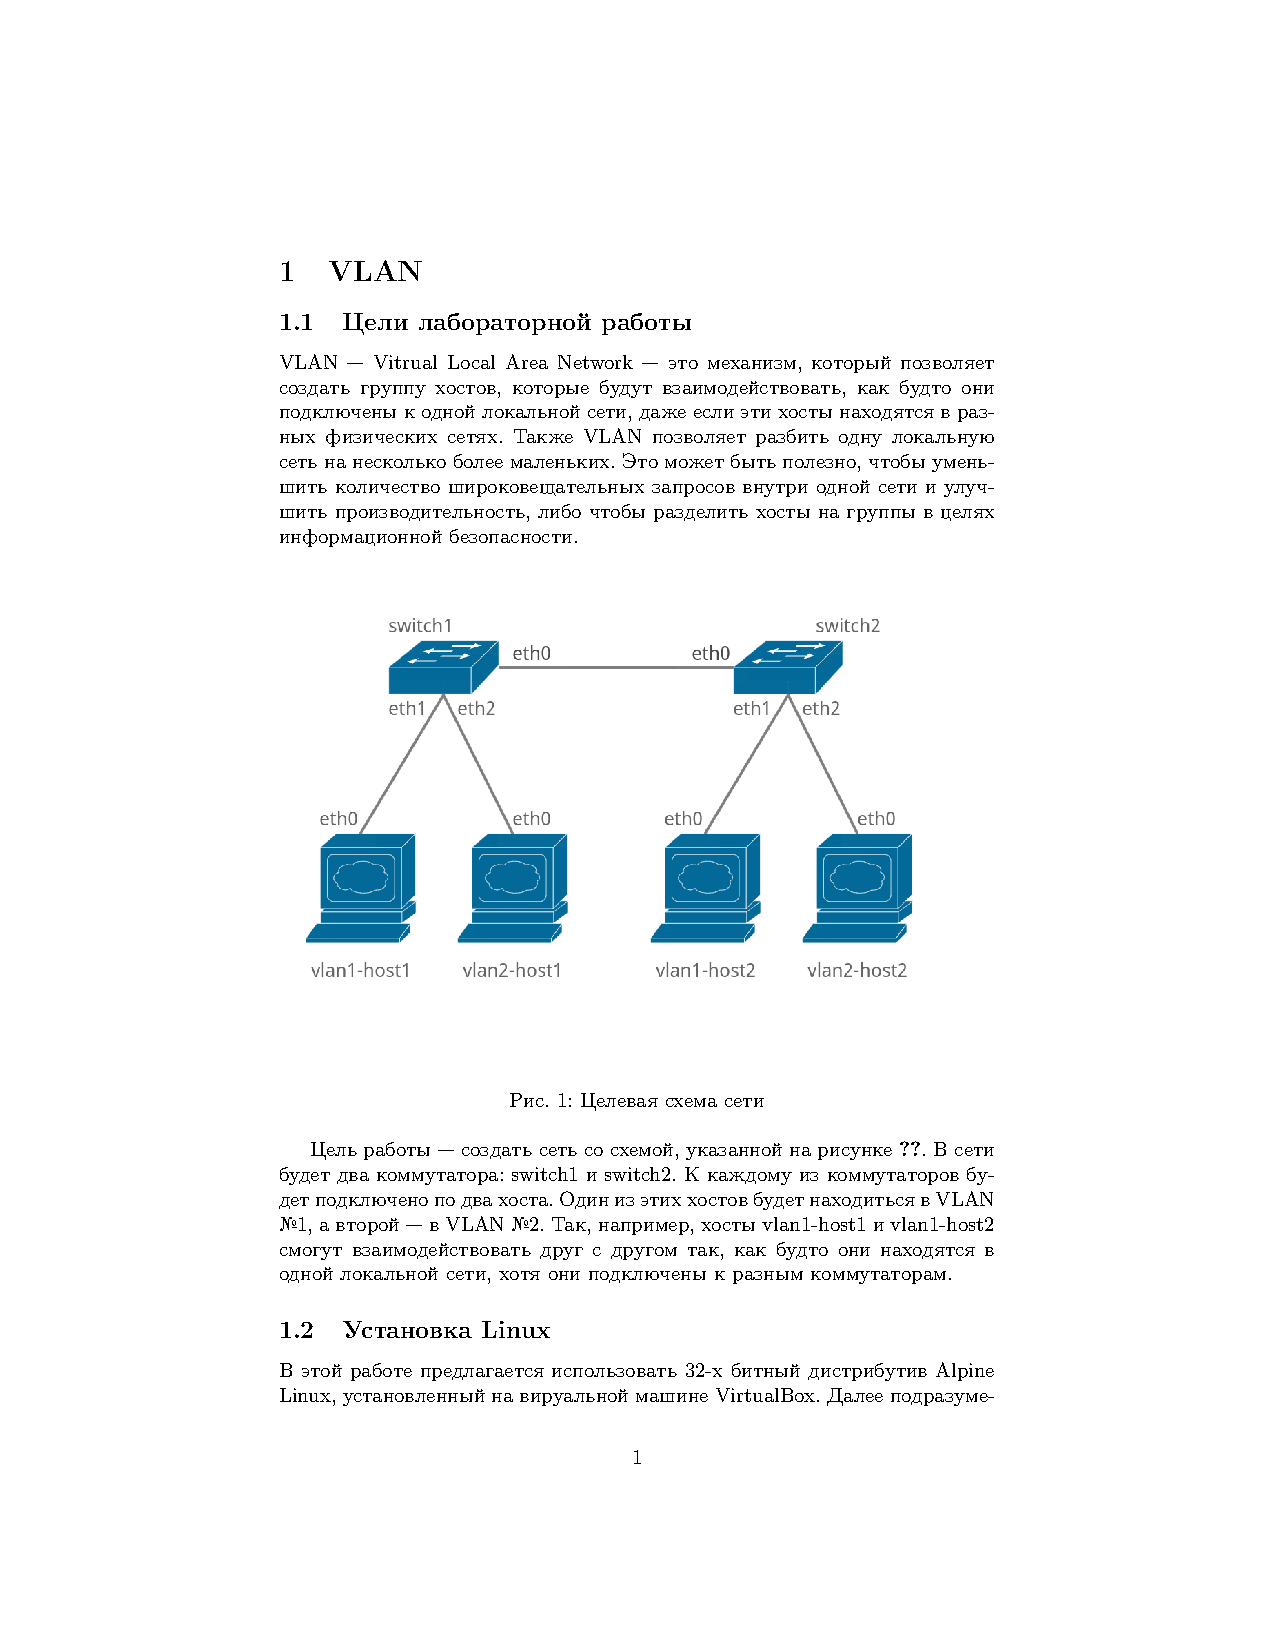
\includegraphics[width=\textwidth]{vlan}
\caption{Целевая схема сети}
\label{vlan-network-configuration}
\end{figure}

Цель работы --- создать сеть со схемой, указанной на рисунке \ref{vlan-network-configuration}. 
В сети будет два коммутатора: switch1 и switch2. К каждому из коммутаторов будет подключено по два хоста. Один из этих хостов будет находиться в VLAN №1, а второй --- в VLAN №2. Так, например, хосты vlan1-host1 и vlan1-host2 смогут взаимодействовать друг с другом так, как будто они находятся в одной локальной сети, хотя они подключены к разным коммутаторам.

\subsection{Установка Linux}
В этой работе предлагается использовать 32-х битный дистрибутив Alpine Linux, установленный на вируальной машине VirtualBox. Далее подразумевается, что начальная настройка виртуальной машины и установка системы уже выполнена.

\subsection{Настройка коммутаторов}
Этот пункт описывает настройку коммутаторов switch1 и switch2. После настройки сетевых адаптеров пропадёт доступ во внешнюю сеть, поэтому сначала на коммутаторы нужно установить необходимые пакеты. 
\begin{itemize}
    \itemsep0em 
    \item Для редактирования файлов нужен текстовый редактор, например vim или nano:
    
    \verb|apk add vim| или \verb|apk add nano|
    \item Для настройки VLAN необходимы пакеты iproute2, bridge и vlan:
    
    \verb|apk add iproute2 bridge vlan|
    \item Для тестирования понадобятся пакеты nmap и iperf3:
    
    \verb|apk add nmap iperf3|
\end{itemize}
После установки пакетов нужно выключить виртуальный машины (команда \verb|poweroff|) и настроить сетевые адаптеры коммутаторов в интерфейсе VirtualBox.

\subsubsection{Настройка сетевых адаптеров в VirtualBox}

\paragraph{Адаптер 1 (eth0).} Этот адаптер будет использоваться как trunk port.
\begin{itemize}
    \itemsep0em 
    \item \emph{Тип подключения}: Внутренняя сеть,
    \item \emph{Имя}: \verb|trunk-net|,
    \item \emph{Неразборчивый режим}: Разрешить всё, 
    \item \emph{Тип адаптера}: Intel PRO/1000 MT Desktop
\end{itemize}
\paragraph{Адаптер 2 (eth1).} Этот адаптер будет использоваться как access port для VLAN №1.
\begin{itemize}
    \itemsep0em 
    \item \emph{Тип подключения}: Внутренняя сеть,
    \item \emph{Имя}: Для switch1 - \verb|switch1-vlan1-net|, для switch2 - \verb|switch2-vlan1-net|
    \item \emph{Неразборчивый режим}: Разрешить всё, 
    \item \emph{Тип адаптера}: Intel PRO/1000 MT Desktop
\end{itemize} 
\paragraph{Адаптер 3 (eth2).} Этот адаптер будет использоваться как access port для VLAN №2.
\begin{itemize}
    \itemsep0em 
    \item \emph{Тип подключения}: Внутренняя сеть,
    \item \emph{Имя}: Для switch1 - \verb|switch1-vlan2-net|, для switch2 - \verb|switch2-vlan2-net|
    \item \emph{Неразборчивый режим}: Разрешить всё, 
    \item \emph{Тип адаптера}: Intel PRO/1000 MT Desktop
\end{itemize}

После настройки сетевых адаптеров в VirtualBox необходимо включить виртуальную машину. 

\subsubsection{Настройка сетевых интерфейсов в Linux}

Для настройки VLAN, нужно отредактировать файл /etc/network/interfaces. Для коммутатора switch1 его содержимое будет таким:
\begin{lstlisting}
auto lo
iface lo inet loopback

auto eth0
iface eth0 inet static
    address 10.0.100.1
    netmask 255.255.255.0
    
iface eth1 inet manual
iface eth2 inet manual

auto vlan100
iface vlan100 inet manual
    vlan-raw-device eth0
    
auto vlan200
iface vlan200 inet manual
    vlan-raw-device eth0

auto br1
iface br1 inet static
    address 192.168.100.1
    netmask 255.255.255.0
    bridge_ports vlan100 eth1
    
auto br2
iface br2 inet static
    address 192.168.200.1
    netmask 255.255.255.0
    bridge_ports vlan200 eth2
\end{lstlisting}
Для коммутатора switch2 будут отличаться только адреса интерфейсов:
\begin{itemize}
    \itemsep0em 
    \item в интерфейсе \verb|eth0| --- \verb|address 10.0.100.2|,
    \item в интерфейсе \verb|br1| --- \verb|address 192.168.100.2|,
    \item в интерфейсе \verb|br2| --- \verb|address 192.168.200.2|,
\end{itemize}
После сохранения файла, нужно применить конфигурацию сетевых интерфейсов командой \verb|/etc/init.d/networking restart|.

\subsection{Настройка хостов}
Этот пункт описывает настройку хостов vlan1-host1, vlan1-host2, vlan2-host1 и vlan2-host2. Перед настройкой сетевого адаптера на каждый хост необходимо установить текстовый редактор и пакеты nmap и iperf3 для тестирования. Затем нужно выключить виртуальную машину и настроить адаптер.

\subsubsection{Настройка сетевого адаптера в VirtualBox}

На каждом хосте нужно сконфигурировать один адаптер VirtualBox:
\begin{itemize}
    \itemsep0em 
    \item \emph{Тип подключения}: Внутренняя сеть,
    \item \emph{Неразборчивый режим}: Разрешить всё, 
    \item \emph{Тип адаптера}: Intel PRO/1000 MT Desktop;
    \item Для каждого хоста необходимо указать имя сети, в которой находится нужный адаптер коммутатора:
    \begin{itemize}
        \itemsep0em 
        \item для vlan1-host1 --- \verb|switch1-vlan1-net|,
        \item для vlan1-host2 --- \verb|switch2-vlan1-net|,
        \item для vlan2-host1 --- \verb|switch1-vlan2-net|,
        \item для vlan2-host2 --- \verb|switch2-vlan2-net|.
    \end{itemize}
\end{itemize}

После настройки сетевых адаптеров в VirtualBox необходимо перезагрузить или включить виртуальную машину. 

\subsubsection{Настройка сетевых интерфейсов в Linux}

На каждом хосте нужно отредактировать файл /etc/network/interfaces. Для хоста vlan1-host1 содержимое файла должно быть таким:

\begin{lstlisting}
auto lo
iface lo inet loopback

auto eth0
iface eth0 inet static
    address 192.168.100.3
    netmask 255.255.255.0
\end{lstlisting}

У остальных хостов файл /etc/network/interfaces заполняется аналогично, изменяя только IP-адрес хоста:
    \begin{itemize}
        \itemsep0em 
        \item для vlan1-host2 --- \verb|address 192.168.100.4|,
        \item для vlan2-host1 --- \verb|address 192.168.200.3|,
        \item для vlan2-host2 --- \verb|address 192.168.200.4|.
    \end{itemize}

В VLAN можно добавить дополнительные хосты. Принадлежность к VLAN определяется портом коммутатора, к которому подключён хост. Для корректной работы сети у каждого из хостов должен быть уникальный IP-адрес. В примере выше IP-адреса задаются вручную, но их можно выдавать и с помощью DHCP.

\subsection{Тестирование}
Тестирование заключается в том, чтобы проверить, что хостам в конкретном VLAN доступны хосты из этого VLAN, но не из другого VLAN. Коммутаторам должны быть доступны хосты в обоих VLAN.

\subsubsection{ping}
Самый примитивный способ протестировать сетевую доступность одного хоста с другого - с помощью команды \verb|ping|.
\begin{lstlisting}
vlan1-host1:~# ping 192.168.100.4
PING 192.168.100.4 (192.168.100.4): 56 data bytes
64 bytes from 192.168.100.4 seq=0 ttl=64 time=5.238 ms
^C
--- 192.168.100.4 ping statistics ---
1 packets transmitted, 1 packets received, 0% packet loss
roud-trip min/avg/max = 6.285/6.285/6.285 ms

vlan1-host1:~# ping 192.168.200.4
PING 192.168.200.4 (192.168.200.4): 56 data bytes
ping: sendto: Network unreachable
\end{lstlisting}

С хоста vlan1-host1 доступен хост vlan1-host2 (192.168.100.4) в VLAN №1, но не доступен vlan2-host2 (192.168.200.4) в VLAN №2

\subsubsection{nmap}
Команда \verb|nmap| позволяет обнаружить хосты, которые находятся в сети. Она пытается пропинговать каждый IP адрес в сети и выводит те, которые ответили.

\begin{lstlisting}
switch1:~# nmap -sP 192.168.200.1/24
Starting Nmap 7.91 ( https://nmap.org ) at 2021-12-19 13:34 UTC
Nmap scan report for 192.168.100.2
Host is up (0.00055s latency).
MAC Address: 08:00:27:A2:42:A4 (Oracle VirtualBox virtual NIC)
Nmap scan report for 192.168.100.3
Host is up (0.00044s latency).
MAC Address: 08:00:27:5E:48:0F (Oracle VirtualBox virtual NIC)
Nmap scan report for 192.168.100.4
Host is up (0.00017s latency).
MAC Address: 08:00:27:F9:D4:97 (Oracle VirtualBox virtual NIC)
Nmap scan report for 192.168.100.1
Host is up.
Nmap done: 256 IP addresses (4 hosts up) scanned in 2.02 seconds

switch1:~# nmap -sP 192.168.200.1/24
Starting Nmap 7.91 ( https://nmap.org ) at 2021-12-19 13:34 UTC
Nmap scan report for 192.168.200.2
Host is up (0.00056s latency).
MAC Address: 08:00:27:AC:31:DE (Oracle VirtualBox virtual NIC)
Nmap scan report for 192.168.200.3
Host is up (0.00025s latency).
MAC Address: 08:00:27:DZ:7A:81 (Oracle VirtualBox virtual NIC)
Nmap scan report for 192.168.200.4
Host is up (0.00023s latency).
MAC Address: 08:00:27:87:F2:72 (Oracle VirtualBox virtual NIC)
Nmap scan report for 192.168.200.1
Host is up.
Nmap done: 256 IP addresses (4 hosts up) scanned in 2.10 seconds
\end{lstlisting}
С коммутатора switch1 доступны по 4 хоста в каждом VLAN (по 2 коммутатора и по 2 обычных хоста). С обычных хостов будут доступны хосты только в одном из VLAN.

\subsubsection{iperf3}
Утилита \verb|iperf3| позволяет проводить тестирование производительности сети между хостами. Для её работы на одном хосте нужно запустить сервер (по умолчанию - на порту 5201) командой \verb|iperf3 -s|, а на другом запустить клиент --- \verb|iperf3 -c <имя или адрес хоста>|. Утилита будет проводить тестирование в течение 10 секунд, затем напечатает отчёт.

\begin{lstlisting}
# Server
vlan2-host2:~# iperf3 -s
------------------------------------------------------------------------
Server listening on 5201 (test #1)
------------------------------------------------------------------------

# Client
vlan2-host1:~# iperf -c 
Connecting to host 192.168.200.4, port 5201
[ 5] local 192.168.200.3 port 37006 connected to 192.168.200.4 port 5201
[ID] Interval         Transfer    Bitrate         Retr  Cwnd
[ 5]  0.00-1.00  sec  141 MBytes  1.18 Gbits/sec  285   303 KBytes
[ 5]  1.00-2.00  sec  128 MBytes  1.07 Gbits/sec   91   438 KBytes
[ 5]  2.00-3.00  sec  143 MBytes  1.20 Gbits/sec  270   298 KBytes
...
[ 5]  9.00-10.00 sec  130 MBytes  1.09 Gbits/sec  135   342 KBytes
- - - - - - - - - - - - - - - - - - - - - - - - - - -
[ID] Interval         Transfer    Bitrate         Retr
[ 5]  0.00-10.00 sec  1.30 GBytes 1.12 Gbits/sec  2001  sender
[ 5]  0.00-10.00 sec  1.30 GBytes 1.12 Gbits/sec        receiver

iperf Done.
\end{lstlisting}
Через сеть между vlan2-host1 и vlan2-host2 можно передавать 1.12 Гигабит в секунду. Если бы клиент и сервер находились на разных хостах, то установить соединение бы не получилось.
\end{document}
